%%%%%%%%%%%%%%%%%%%%%%%%%%%%%%%%%%%%%%%%%%%%%%%%%%%%%%%%%%%%%%%%%%%%%%%%%%%%%%%%%%
\begin{frame}[fragile]\frametitle{}
\begin{center}
{\Large Dimensionality of Data}
\end{center}
\end{frame}


%%%%%%%%%%%%%%%%%%%%%%%%%%%%%%%%%%%%%%%%%%%%%%%%%%%%%%%%%%%
\begin{frame}[fragile]\frametitle{These days...}
	\begin{itemize}
	\item Data Deluge: Internet, Social Media and IoT. 
	\item 4Vs : Volume - Velocity - Variety - Veracity. 
	\end{itemize}
\end{frame}

%%%%%%%%%%%%%%%%%%%%%%%%%%%%%%%%%%%%%%%%%%%%%%%%%%%%%%%%%%%
\begin{frame}[fragile]\frametitle{Data Redundancy}
	\begin{itemize}
	\item One parameter measured multiple times, multiple ways
	\item Example: A motorbike rider in racing competitions
	\begin{itemize}
	\item GPS Sensors for Position and movement
	\item Gyro meters,  video feeds , smart watch. 
	\item Data not matching exactly.
	\item Little incremental. 
	\end{itemize}
	\item Need to extract core parameters
	\end{itemize}
\end{frame}

%%%%%%%%%%%%%%%%%%%%%%%%%%%%%%%%%%%%%%%%%%%%%%%%%%%%%%%%%%%
\begin{frame}[fragile]\frametitle{Why high Dimensionality is a problem? }
Because most Machine Learning methods are statistical, meaning:
	\begin{itemize}
	\item Count observations, different classes. 
	\item Say decision tree counts labels.
	\end{itemize}
\end{frame}

%%%%%%%%%%%%%%%%%%%%%%%%%%%%%%%%%%%%%%%%%%%%%%%%%%%%%%%%%%%
\begin{frame}[fragile]\frametitle{Why high Dimensionality is a problem? }
	\begin{itemize}
	\item 10 data points
	\item Each with 3 possible values
	\item Single x axis. 
	\item Lower values on lower side, etc.
	\end{itemize}
\begin{center}
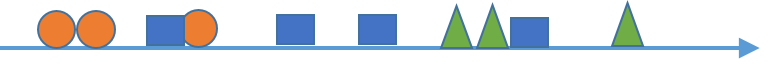
\includegraphics[width=0.5\linewidth,keepaspectratio]{1d}
\end{center}
\tiny{(Reference: Principal Component Analysis - Victor Lavrenko)}
\end{frame}

%%%%%%%%%%%%%%%%%%%%%%%%%%%%%%%%%%%%%%%%%%%%%%%%%%%%%%%%%%%
\begin{frame}[fragile]\frametitle{Why high Dimensionality is a problem? }
	\begin{itemize}
	\item One dimension is added 
	\item Each data point represented by two dimensions: $(x_1, x_2)$ both having 3 values.
	\item 10 points will be $3^2 = 9$ regions
	\end{itemize}
\begin{center}
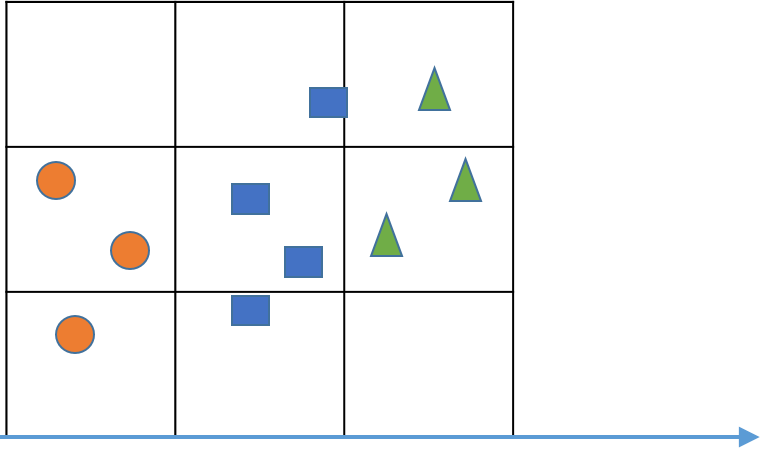
\includegraphics[width=0.5\linewidth,keepaspectratio]{2d}
\end{center}	
Some regions with no data points. 
\tiny{(Reference: Principal Component Analysis - Victor Lavrenko)}
\end{frame}

%%%%%%%%%%%%%%%%%%%%%%%%%%%%%%%%%%%%%%%%%%%%%%%%%%%%%%%%%%%
\begin{frame}[fragile]\frametitle{Why high Dimensionality is a problem? }
	\begin{itemize}
	\item Sparseness grows more with more dimensions
	\item Density reduces
	\end{itemize}
\begin{center}
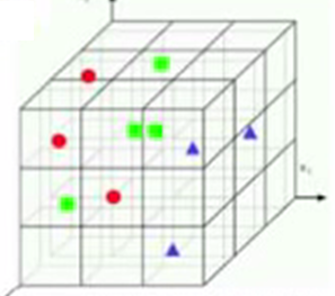
\includegraphics[width=0.5\linewidth,keepaspectratio]{3d}
\end{center}	
\tiny{(Reference: Principal Component Analysis - Victor Lavrenko)}
\end{frame}

%%%%%%%%%%%%%%%%%%%%%%%%%%%%%%%%%%%%%%%%%%%%%%%%%%%%%%%%%%%
\begin{frame}[fragile]\frametitle{The curse}
	\begin{itemize}
	\item High dimensionality : Less query performance 
	\item More processing power 
	\item More storage.  
	\item That's the curse of dimensionality
	\end{itemize}
\end{frame}

%%%%%%%%%%%%%%%%%%%%%%%%%%%%%%%%%%%%%%%%%%%%%%%%%%%%%%%%%%%
\begin{frame}[fragile]\frametitle{Purpose of Dimension reduction}
	\begin{itemize}
	\item To discover smaller ``intrinsic'' Dimensionality
	\item Visualization: Projection of High dimensions to 2D or 3D. 
	\item Data compression for an efficient storage and retrieval
	\item Regression or classification more accurate in reduced space
	\item Noise removal for better clustering, pattern recognition
	\end{itemize}
\end{frame}

%%%%%%%%%%%%%%%%%%%%%%%%%%%%%%%%%%%%%%%%%%%%%%%%%%%%%%%%%%%%
%\begin{frame}[fragile]\frametitle{Applications of dimension reduction}
%Face recognition, Handwritten digit recognition
%\begin{center}
%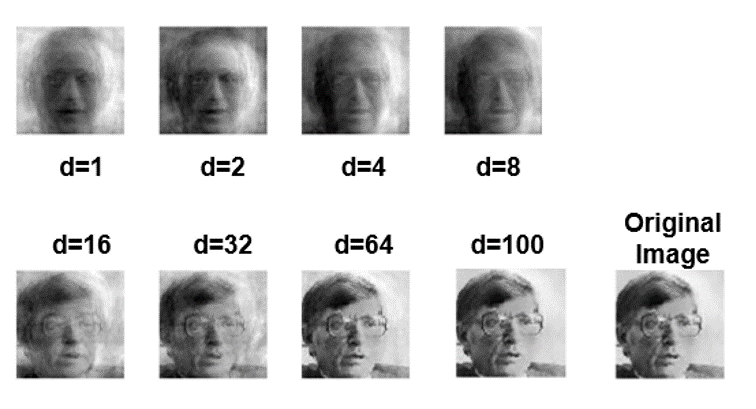
\includegraphics[width=0.7\linewidth,keepaspectratio]{face}
%\end{center}		
%\end{frame}


%%%%%%%%%%%%%%%%%%%%%%%%%%%%%%%%%%%%%%%%%%%%%%%%%%%%%%%%%%%
\begin{frame}[fragile]\frametitle{Applications of dimension reduction}
	\begin{itemize}
	\item Information Retrieval: Web documents(Text,  Images) 
	\item Recommender System: Large rating matrix 
	\item Social Networks: Facebook graph millions of users 
	\end{itemize}
\end{frame}




%%%%%%%%%%%%%%%%%%%%%%%%%%%%%%%%%%%%%%%%%%%%%%%%%%%%%%%%%%%
\begin{frame}[fragile]\frametitle{Conclusions}
	\begin{itemize}
	\item Dimension Reduction is the need of the hour
	\item Not losing important features is the key
	\item Knowledge of domain, statistics and usage of various techniques can help in the task
	\end{itemize}
\end{frame}

